\subsection{Circuito II: VFA-CFA}
\hspace{1mm} El amplificador operacional que se implementa para el circuito propuesto es el LM6181 (CFA) cuyas especificaciones se detallan a continuación.

\begin{itemize}[itemsep=1pt]
    \item \(R_T=2.37~M\Omega\)
    \item \(C_T=4.8~pF\)
    \item \(F_1=14~KHz\)
    \item \(F_2=82.3~MHz\)
\end{itemize}

\bigskip
\hspace{1mm} Se considera que el amplificador operacional LM324 (VFA) se comporta de la misma manera que en el caso anterior  y que el polo de mayor frecuencia del CFA tiene un efecto despreciable sobre la respuesta del amplificador a lazo cerrado.

\bigskip
\hspace{1mm} La ecuación de margen de fase para máxima planicidad de módulo se desarrolla de la siguiente manera:

\begin{equation}
    M \varphi = 360^o - 180^o - arctg \left(\frac{f_g}{f_{1VFA}}\right) - arctg \left(\frac{f_g}{f_{2VFA}}\right) - arctg \left(\frac{f_g}{f_{CFA}}\right) = 65,5^o
\end{equation}

\bigskip
\hspace{1mm} Reemplazando por los valores dados.

\begin{equation}
    65,5^o = 180^o - arctg \left(\frac{2~MHz}{10~Hz}\right) - arctg \left(\frac{2~MHz}{5,06~MHz}\right) - arctg \left(\frac{2~MHz}{f_{CFA}}\right)
\end{equation}
\begin{equation}
    65,5^o = 180^o - 90^o - 21,57^o - arctg \left(\frac{2~MHz}{f_{CFA}}\right)
\end{equation}

\begin{equation}
    arctg\left(\frac{2~MHz}{f_{CFA}}\right) = 180^o - 90^o - 21,57^o - 65,5^o
\end{equation}
\begin{equation}
    arctg\left(\frac{2~MHz}{f_{CFA}}\right) = 2,93^o
\end{equation}
\begin{equation}
    tg (2,93^o) = \frac{2~MHz}{f_{CFA}}
\end{equation}
\bigskip
\hspace{1mm}Se tiene que la frecuencia del polo generado por el amplificador CFA es la siguiente:
\begin{equation}
    f_{CFA} = \frac{2~MHz}{tg (2,93^o)} = 39~MHz
\end{equation}
\bigskip
\hspace{1mm} Para obtener una máxima planicidad de módulo, la frecuencia del polo de lazo cerrado del CFA debe ser.
\begin{equation}
    \boxed{
        f_{CFA} = 39~MHz
    }
\end{equation}
\bigskip
\hspace{1mm} Como se conoce la frecuencia del amplificador CFA \((f_{CFA})\) . Se calcula la resistencia \( R_2 \) partiendo de la siguiente fórmula.
\begin{equation}
    \omega _{CFA} = \frac{1}{C_T \cdot R_2}
\end{equation}
\begin{equation}
    R_2 = \frac{1}{C_T \cdot 2\pi f_{CFA}} = \frac{1}{4,8~pF \cdot 2\pi \cdot 39~MHz}
\end{equation}
\begin{equation}
    \boxed{
        R_2 = 850~\Omega
    }
\end{equation}
\bigskip
\hspace{1mm} Se calcula la resistencia \( R_1 \) . En primera instancia, se calcula la ganancia Avf2.
\begin{equation}
    Avf \cdot f_g = Ado \cdot f_1 \cdot Avf_2
\end{equation}
\bigskip
\hspace{1mm} Se calcula la ganancia ideal de lazo cerrado del amplificador CFA \(( Avf_2)\). Se despeja la misma de la fórmula anterior.

\begin{equation}
    Avf_2 = \frac{Avf \cdot f_g}{Ado \cdot f_1} = \frac{10 \cdot 2~MHz}{100000 \cdot 10~Hz}
\end{equation}
\begin{equation}
    \boxed{
    Avf_2 = 20
    }
\end{equation}
\bigskip
\hspace{1mm} Finalmente, se calculará \( R_1 \) partiendo de la siguiente ecuación.

\begin{equation}
    Avf_2 = \Bigl(1 + \frac{R_2}{R_1}\Bigl) = 20
\end{equation}
\begin{equation}
    \frac{R_2}{R_1} = 20-1
\end{equation}
\begin{equation}
    R_1 =\frac{R_2}{19}
\end{equation}
\begin{equation}
    R_1 =\frac{850\Omega}{19}
\end{equation}
\begin{equation}
    R_1 =44,73\Omega \approx 45\Omega
\end{equation}
\begin{equation}
    \boxed{
    R_1 =45\Omega
    }
\end{equation}
\bigskip
\hspace{1mm} Como se vio en el marco teórico, al trabajar en máxima planicidad de módulo la frecuencia del polo de la función de transferencia a lazo cerrado se obtiene a partir de la siguiente expresión.

\begin{equation}
    \omega _G = 0,644 \cdot \omega _p 
\end{equation}

\bigskip
\hspace{1mm} Se especifica para el diseño que el ancho de banda potencial que se requiere es de \( f_G = 2~MHz \). Por lo tanto reemplazando y despejando de la ecuación anterior \( f_p \).

\begin{equation}
    2\pi f_G = 0,644 \cdot 2\pi f_p \Longrightarrow f_p = \frac{f_G}{0,644} = \frac{2~MHz}{0,644}
\end{equation}

\begin{equation}
    \boxed{
    f_p = 3,1~MHz
    }
\end{equation}

\bigskip
\hspace{1mm} El ancho de banda a -3dB es igual a la frecuencia del polo a lazo cerrado, que en este caso es de 3.1 MHz, ya que esta es una condición que busca maximizar la planicidad del módulo.

\subsubsection{Simulaciones}

\hspace{1mm} Se realizó la simulación del circuito propuesto en el software LTSpice. Se tiene para este caso que se implementan los amplificadores operacionales LM324 (VFA) y LM6181 (CFA).
\begin{figure}[!h]
    \centering
    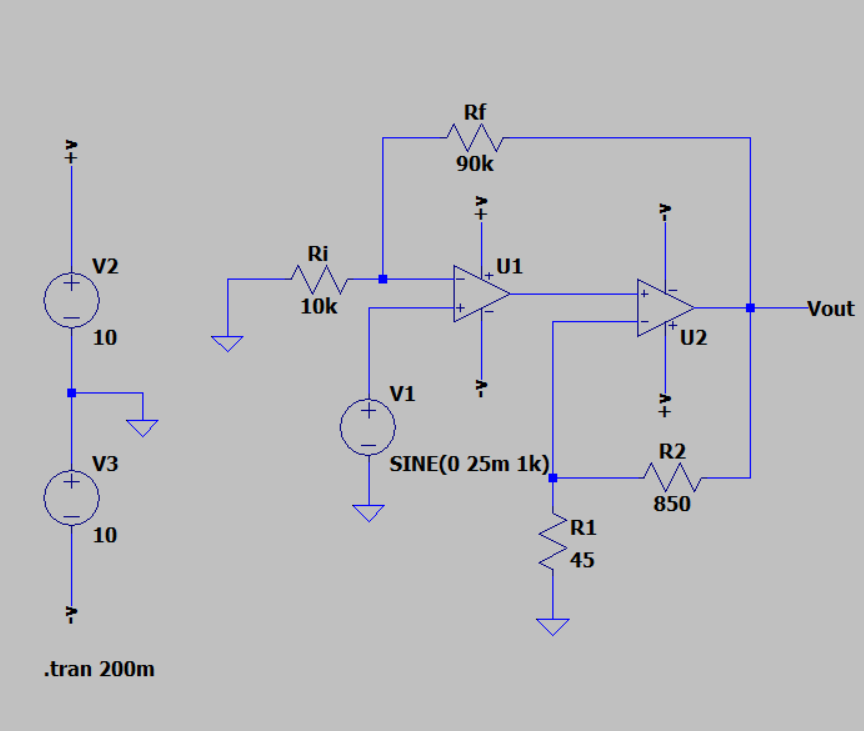
\includegraphics[width=0.6\linewidth]{VFA - CFA/Imágenes/Circuito 2 - VFA CFA.png}
    \caption{Amplificador VFA-CFA}
    
\end{figure}
    
\hspace{1mm} Se inyectó una señal sinusoidal con un valor de tensión pico de \(25~mV\) con una frecuencia de \( 1~kHz \).  Se obtienen las siguientes mediciones.
\begin{figure}[!h]
    \centering
    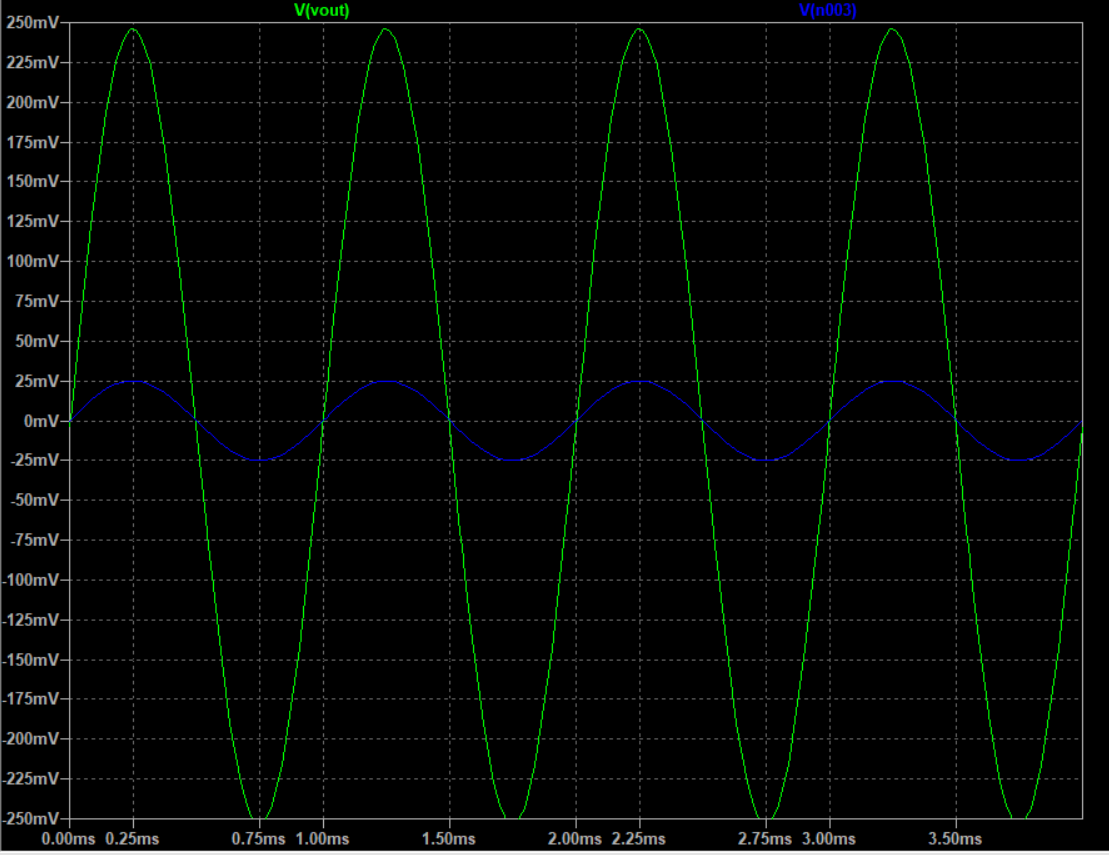
\includegraphics[width=0.6\linewidth]{VFA - CFA/Imágenes/Circuito 2 - Simulación.png}
    \caption{Ganancia del Amplificador Compuesto.}
\end{figure}
\hspace{1mm} En donde se puede comprobar que para un valor de entrada de \( 25~mV \) se obtiene a la salida \( 94.125~mV \) con lo cual la ganancia obtenida es.

\begin{equation}
    G = \frac{250~mV}{25~mV}
\end{equation}
\begin{equation}
    \boxed{
    G = 10
    }
\end{equation}

\hspace{1mm} Se realiza el diagrama de bode del circuito propuesto. 
\begin{figure}[!h]
    \centering
    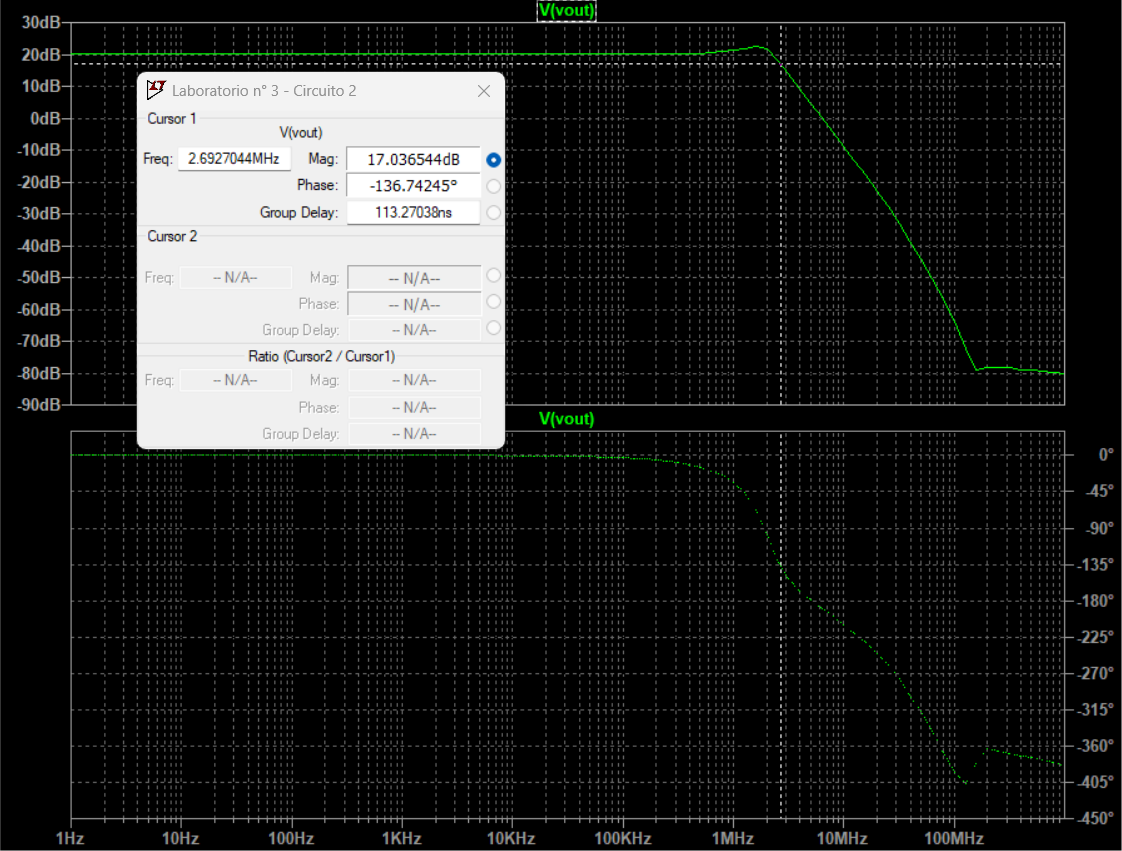
\includegraphics[width=0.7\linewidth]{VFA - CFA/Imágenes/Circuito 2 - Amplitud y Fase.png}
    \caption{Diagrama de Bode.}
\end{figure}
\hspace{1mm} Se observa una ganancia de \(20~dB\) y una caída de \(-3~dB\) a la frecuencia de \(2.7~MHz\).






